\documentclass[10pt,twocolumn]{article}

\usepackage[utf8]{inputenc}
\usepackage[T1]{fontenc}
\usepackage[french]{babel}
\usepackage{graphicx}
\usepackage{amsmath}
\usepackage{booktabs}
\usepackage{hyperref}
\usepackage{caption}
\usepackage[margin=2cm]{geometry}

\title{ViT vs CNN : une étude comparative sur classification fine-grained}
\author{
  Prénom Nom A \and Prénom Nom B \and Prénom Nom C \\
  M1 IA — ESGIS
}
\date{\today}

\begin{document}

\twocolumn[
  \begin{@twocolumnfalse}
    \maketitle
    \begin{abstract}
    % Résumé à rédiger en dernier, une fois les résultats disponibles (~150-200 mots).
    % Doit couvrir : problème traité, méthode, résultats principaux, conclusion.
    TODO: résumé.
    \end{abstract}
    \vspace{1em}
  \end{@twocolumnfalse}
]

\section{Introduction}
\label{sec:introduction}

% Rôle C — à rédiger (~0.75-1 page)
%
% Points à couvrir :
% - Contexte : classification fine-grained (distinguer des sous-catégories
%   visuellement très proches, ex. espèces d'oiseaux).
% - Pourquoi c'est difficile : faibles différences inter-classes,
%   variabilité intra-classe (pose, éclairage, arrière-plan).
% - Les deux familles d'architectures comparées : CNN (ResNet-50, biais
%   inductif de localité/convolution) vs ViT (self-attention, moins de
%   biais inductif, réputé plus data-hungry).
% - Question de recherche du projet : comment ces deux architectures se
%   comportent-elles sur CUB-200-2011, notamment en fonction de la
%   quantité de données disponibles (courbe data-hungry) ?
% - Annoncer le plan du rapport.

TODO: rédiger l'introduction.

\section{Travaux liés}
\label{sec:related_work}

\paragraph{Réseaux convolutifs pour la classification d'images.}
Les architectures convolutives profondes, dont ResNet~\cite{he2016resnet},
ont longtemps constitué l'approche dominante en classification d'images.
Leur biais inductif de localité (les filtres convolutifs traitent des
voisinages de pixels) et d'invariance par translation les rend
particulièrement efficaces sur des jeux de données de taille modeste,
puisque ce biais réduit l'espace des hypothèses que le modèle doit
apprendre directement à partir des données.

\paragraph{Vision Transformers.}
Dosovitskiy et al.~\cite{dosovitskiy2020vit} introduisent le Vision
Transformer (ViT), qui découpe une image en une grille de patches traités
comme une séquence de tokens, à la manière d'un Transformer pour le texte.
Contrairement aux CNN, le ViT ne possède aucun biais inductif de localité
intégré à l'architecture : les relations spatiales entre patches doivent
être entièrement apprises à partir des données via les mécanismes
d'auto-attention. Les auteurs montrent que le ViT peut surpasser les CNN
à condition d'être pré-entraîné sur des jeux de données massifs
(centaines de millions d'images), mais qu'il performe nettement moins
bien que les CNN lorsqu'il est entraîné from scratch sur des jeux de
données de taille modeste — le ViT est ainsi qualifié de plus
\emph{data-hungry}.

\paragraph{DeiT et l'efficacité en données.}
Touvron et al.~\cite{touvron2021deit} (DeiT) abordent directement cette
limite en proposant une stratégie d'entraînement — notamment une
distillation par un modèle enseignant convolutif — permettant d'entraîner
des ViT compétitifs sur ImageNet sans recourir à un pré-entraînement sur
des données massives. Ce travail est particulièrement pertinent pour ce
projet : il documente empiriquement le comportement data-hungry des ViT
et propose des pistes pour l'atténuer, ce qui motive directement l'analyse
de sensibilité à la quantité de données menée en
Section~\ref{sec:ablation} (courbe d'accuracy en fonction de la fraction
du jeu d'entraînement utilisée).

\paragraph{Classification fine-grained.}
La classification fine-grained pose des difficultés spécifiques par
rapport à la classification générique : les catégories partagent une
structure globale similaire et ne se distinguent que par des détails
localisés. Le jeu de données CUB-200-2011~\cite{wah2011cub}, utilisé dans
ce projet, est une référence classique pour évaluer les architectures sur
ce type de tâche.

\paragraph{Positionnement de ce projet.}
Ce projet se situe à l'intersection de ces travaux : il reproduit à petite
échelle une comparaison ViT vs CNN sur une tâche fine-grained, en mettant
l'accent sur la sensibilité de chaque architecture à la quantité de
données disponible plutôt que sur la seule performance finale.
\section{Méthode}
\label{sec:methodology}

\subsection{Architectures}

Trois architectures sont comparées, toutes adaptées à la classification
sur les 200 classes de CUB-200-2011 :

\begin{itemize}
  \item \textbf{ResNet-50 pré-entraîné} : backbone \texttt{torchvision}
    pré-entraîné sur ImageNet, dont la dernière couche entièrement
    connectée est remplacée par une couche linéaire à 200 sorties.
  \item \textbf{ViT pré-entraîné} : backbone \texttt{timm}
    (\texttt{vit\_small\_patch16\_224} ou \texttt{vit\_small\_patch32\_224}
    selon la taille de patch), pré-entraîné sur ImageNet, avec une tête
    de classification à 200 sorties.
  \item \textbf{ViT from scratch} : implémentation entièrement codée pour
    ce projet, sans pré-entraînement. L'image est découpée en patches
    (16 ou 32 pixels) projetés linéairement (\emph{patch embedding}), un
    token \texttt{[CLS]} est ajouté à la séquence, un encodage
    positionnel appris est additionné, puis la séquence traverse 6
    blocs Transformer (dimension d'embedding 384, 6 têtes d'attention,
    ratio MLP de 4). La classification finale s'appuie sur le token
    \texttt{[CLS]} après normalisation.
\end{itemize}

\subsection{Protocole d'entraînement}

Chaque modèle est entraîné avec l'optimiseur AdamW (taux d'apprentissage
$10^{-4}$, weight decay $0{,}01$), une fonction de perte d'entropie
croisée, une taille de batch de 32, sur 3 epochs. Les images sont
prétraitées et augmentées selon les pipelines décrits en
Section~\ref{sec:data} (redimensionnement à 224$\times$224,
normalisation ImageNet, augmentation faible par défaut). Les
variantes ResNet-50 et ViT from scratch sont également entraînées sur
les sous-ensembles à 10\,\%, 25\,\% et 50\,\% du jeu d'entraînement
complet, dans les mêmes conditions, pour l'analyse de sensibilité à la
quantité de données (Section~\ref{sec:ablation}).

Le meilleur modèle de chaque run est sélectionné selon l'accuracy de
validation et sauvegardé automatiquement à chaque amélioration.

\subsection{Limite du protocole actuel}

Le nombre d'epochs (3) a été fixé pour des raisons de temps de calcul
disponible sur la durée du projet. Cette contrainte affecte
particulièrement le ViT from scratch, qui ne bénéficie d'aucun
pré-entraînement et nécessite un nombre d'itérations nettement plus
élevé pour converger, en cohérence avec son comportement data-hungry
documenté en Section~\ref{sec:related_work}. Un scheduler de taux
d'apprentissage, l'entraînement en précision mixte et un mécanisme
d'arrêt anticipé ont été implémentés dans l'outil d'entraînement du
projet mais n'ont pas encore été appliqués aux résultats rapportés
ici ; cette limite est reprise en Section~\ref{sec:discussion}.
\section{Données}
\label{sec:data}

\subsection{Jeu de données}

Le jeu de données utilisé est CUB-200-2011~\cite{wah2011cub}
(Caltech-UCSD Birds), qui comprend 11\,788 images réparties sur 200
espèces d'oiseaux. La distribution du nombre d'images par classe est
légèrement déséquilibrée, avec un minimum de 41 images et un maximum de 60
images par classe (Figure~\ref{fig:class_distribution}), ce qui ne
nécessite pas de pondération de classes particulière. Les images ont une
résolution native moyenne de 471$\times$384 pixels, avec une variabilité
notable (de 140 à 500 pixels de large selon les images), ce qui justifie
le choix d'un redimensionnement systématique à 224$\times$224 pixels pour
l'entraînement.

\begin{figure}[t]
  \centering
  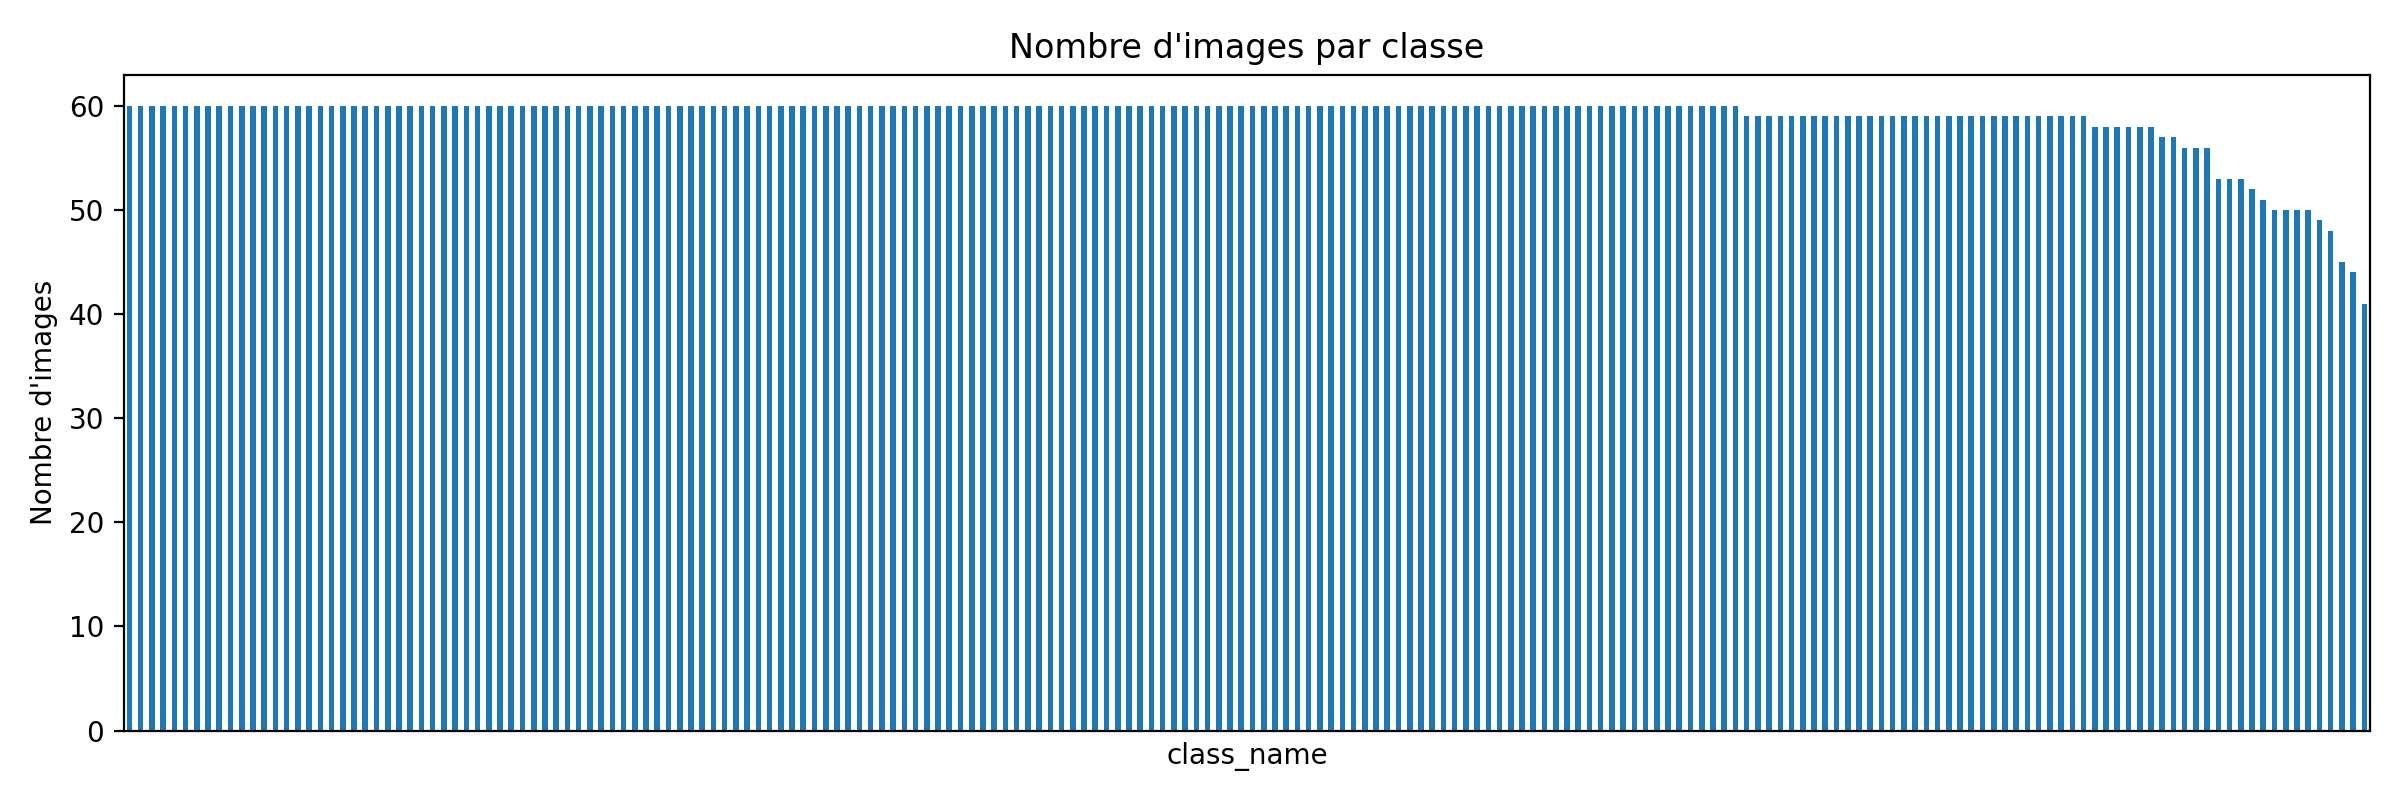
\includegraphics[width=\linewidth]{../data/data_processed/figures/eda_class_distribution.png}
  \caption{Distribution du nombre d'images par classe sur CUB-200-2011.}
  \label{fig:class_distribution}
\end{figure}

La Figure~\ref{fig:similar_classes} illustre la difficulté propre à la
classification fine-grained : plusieurs espèces de moineaux (\emph{Baird
Sparrow}, \emph{Black-throated Sparrow}, \emph{Brewer Sparrow},
\emph{Chipping Sparrow}) partagent une silhouette et une taille très
proches, et ne se distinguent que par des détails de plumage.

\begin{figure}[t]
  \centering
  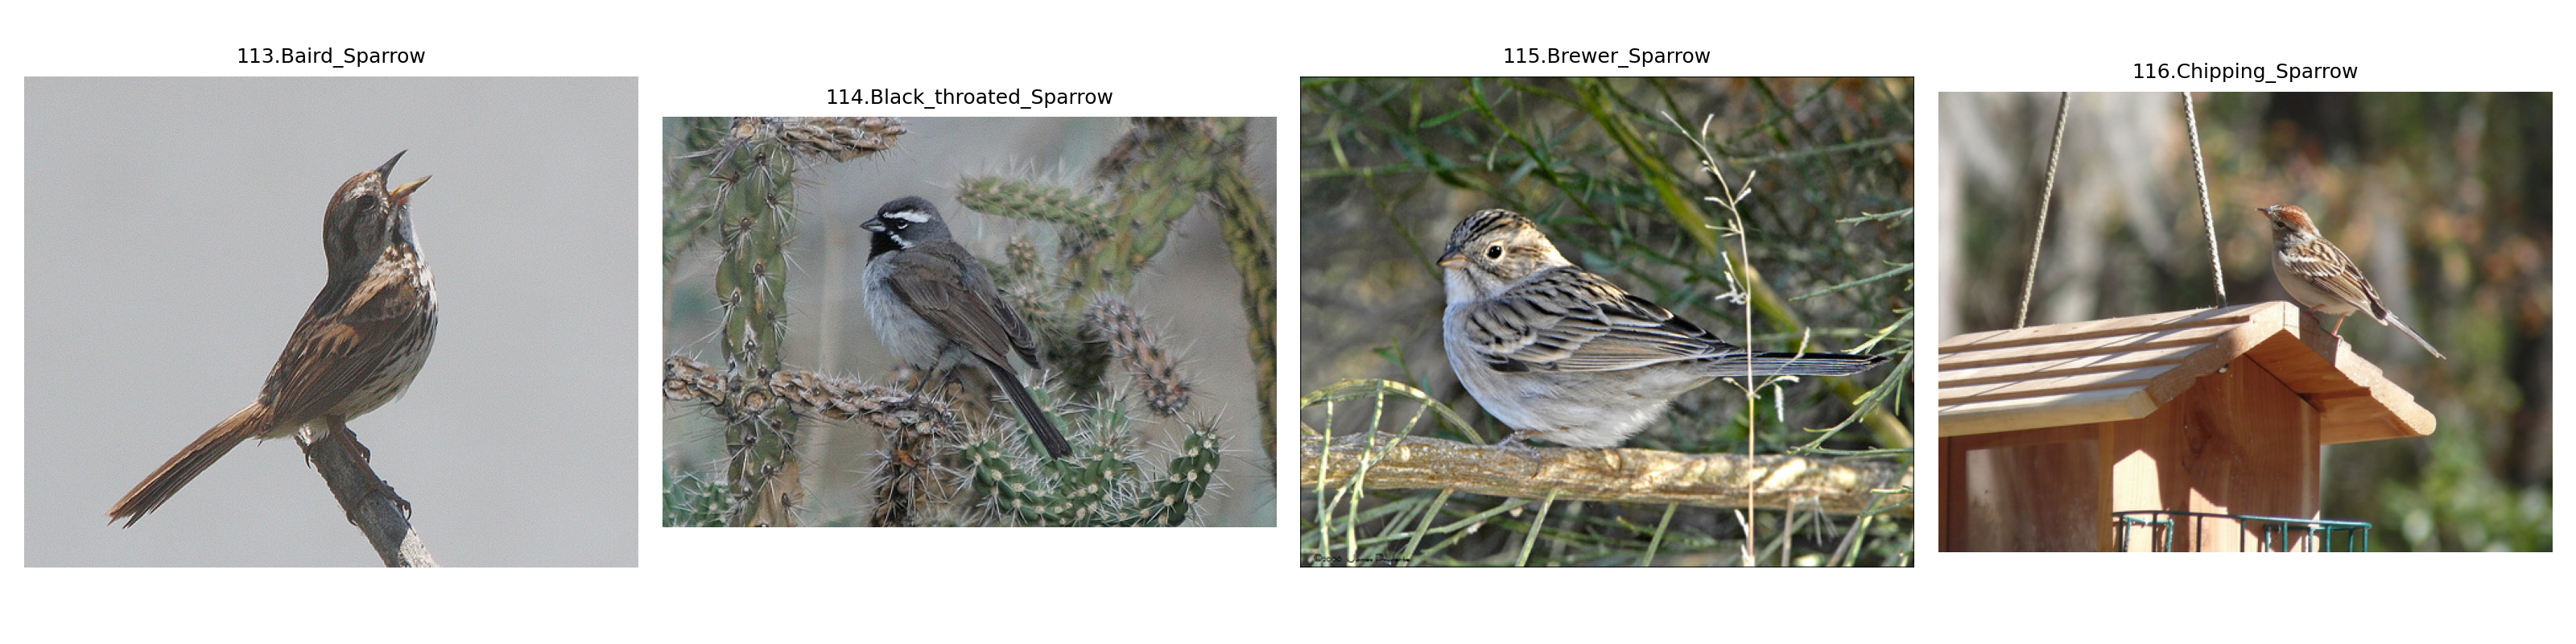
\includegraphics[width=\linewidth]{../data/data_processed/figures/eda_similar_classes.png}
  \caption{Exemple de classes visuellement proches (famille des moineaux), illustrant la difficulté du fine-grained.}
  \label{fig:similar_classes}
\end{figure}

\subsection{Prétraitement}

Toutes les images sont redimensionnées à 224$\times$224 pixels et
normalisées avec les statistiques d'ImageNet (moyenne et écart-type par
canal RGB), afin d'assurer la compatibilité avec les modèles
pré-entraînés utilisés (Section~\ref{sec:methodology}).

\subsection{Séparation train / validation / test}

Le split officiel de CUB-200-2011 fournit une séparation
train/test de 5\,994 / 5\,794 images. À partir de l'ensemble
d'entraînement officiel, un sous-ensemble de validation stratifié de
15\,\% est extrait (seed fixe = 42), aboutissant à la répartition finale
suivante :

\begin{table}[t]
  \centering
  \caption{Répartition finale des images par split.}
  \label{tab:splits}
  \begin{tabular}{lc}
    \toprule
    Split & Nombre d'images \\
    \midrule
    Train & 5\,094 \\
    Validation & 900 \\
    Test & 5\,794 \\
    \midrule
    Total & 11\,788 \\
    \bottomrule
  \end{tabular}
\end{table}

\subsection{Sous-échantillonnage pour l'analyse data-hungry}

Afin d'étudier la sensibilité de chaque architecture à la quantité de
données d'entraînement (Section~\ref{sec:ablation}), quatre
sous-ensembles stratifiés de l'ensemble d'entraînement sont générés,
correspondant à 10\,\%, 25\,\%, 50\,\% et 100\,\% des 5\,094 images de
train (seed fixe = 42, toutes les 200 classes restant représentées même
dans le sous-ensemble à 10\,\%).

\subsection{Augmentation des données}

Deux pipelines d'augmentation sont définis pour l'entraînement : un
pipeline \emph{faible} (retournement horizontal aléatoire, recadrage
aléatoire léger) et un pipeline \emph{fort} (ajout d'une variation
colorimétrique, d'une rotation aléatoire et d'un effacement aléatoire de
zones de l'image). Aucune augmentation n'est appliquée sur les ensembles
de validation et de test.
\section{Étude d'ablation}
\label{sec:ablation}

\subsection{Comparaison des configurations}

Le Tableau~\ref{tab:ablation} présente les résultats de test (top-1,
top-5, perte, nombre de paramètres) pour les 12 configurations
entraînées : ResNet-50 (jeu complet et sous-échantillons), ViT
pré-entraîné (patch16 et patch32), et ViT entraîné from scratch (jeu
complet et sous-échantillons, patch16 et patch32).

\begin{table}[t]
  \centering
  \caption{Résultats de test pour l'ensemble des configurations entraînées.}
  \label{tab:ablation}
  \small
  \begin{tabular}{lccc}
    \toprule
    Configuration & Top-1 & Top-5 & Params \\
    \midrule
    ResNet-50 (100\,\%)          & 71{,}9\,\% & 93{,}6\,\% & 23{,}9M \\
    ResNet-50 (50\,\%)           & 48{,}7\,\% & 81{,}1\,\% & 23{,}9M \\
    ResNet-50 (25\,\%)           & 23{,}5\,\% & 48{,}9\,\% & 23{,}9M \\
    ResNet-50 (10\,\%)           & 5{,}1\,\%  & 14{,}0\,\% & 23{,}9M \\
    \midrule
    ViT pré-entraîné (patch32)   & 53{,}9\,\% & 83{,}5\,\% & 22{,}6M \\
    ViT pré-entraîné (patch16)   & 9{,}9\,\%  & 25{,}4\,\% & 21{,}7M \\
    \midrule
    ViT scratch (100\,\%)        & 1{,}1\,\%  & 4{,}8\,\%  & 11{,}1M \\
    ViT scratch (50\,\%)         & 2{,}2\,\%  & 7{,}1\,\%  & 11{,}1M \\
    ViT scratch (25\,\%)         & 1{,}0\,\%  & 4{,}9\,\%  & 11{,}1M \\
    ViT scratch (10\,\%)         & 1{,}1\,\%  & 4{,}5\,\%  & 11{,}1M \\
    ViT scratch (patch16, sans aug.) & 2{,}1\,\% & 9{,}0\,\% & 11{,}1M \\
    ViT scratch (patch32)        & 2{,}0\,\%  & 8{,}5\,\%  & 11{,}9M \\
    \bottomrule
  \end{tabular}
\end{table}

\subsection{Sensibilité à la quantité de données}

La Figure~\ref{fig:data_hungry} illustre la sensibilité de ResNet-50 et
du ViT from scratch à la fraction du jeu d'entraînement utilisée.
ResNet-50 présente une croissance monotone et régulière de
l'accuracy avec la quantité de données (5{,}1\,\% à 10\,\%, jusqu'à
71{,}9\,\% à 100\,\%), cohérente avec son biais inductif convolutif qui
lui permet d'extraire une structure utile même à partir de peu
d'exemples. Le ViT from scratch, à l'inverse, reste bloqué à un niveau
proche du hasard (0{,}5\,\% attendu pour 200 classes) quelle que soit
la fraction de données utilisée, sans amélioration significative entre
10\,\% et 100\,\%.

\begin{figure}[t]
  \centering
  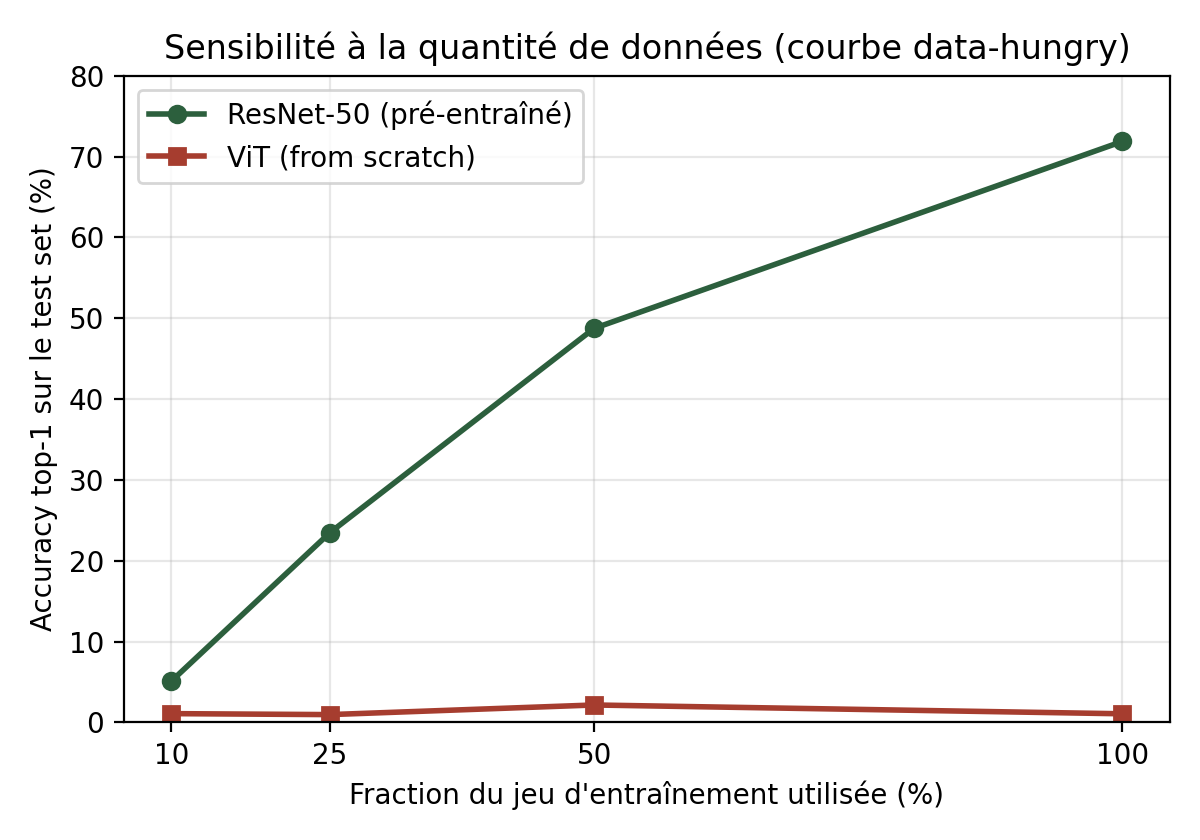
\includegraphics[width=\linewidth]{figures/data_hungry_curve.png}
  \caption{Accuracy top-1 en fonction de la fraction du jeu d'entraînement utilisée, pour ResNet-50 et le ViT from scratch.}
  \label{fig:data_hungry}
\end{figure}

\subsection{Discussion des résultats}

Trois observations principales se dégagent de cette étude d'ablation.

\textbf{Le pré-entraînement est déterminant pour le ViT.} Le ViT
pré-entraîné sur ImageNet (variante patch32) atteint 53{,}9\,\% de
top-1, largement au-dessus du ViT from scratch, quelle que soit la
quantité de données d'entraînement disponible pour ce dernier. Ce
résultat confirme empiriquement, sur CUB-200-2011, le comportement
data-hungry du ViT documenté par Dosovitskiy et al.~\cite{dosovitskiy2020vit}
et discuté par Touvron et al.~\cite{touvron2021deit} : sans
pré-entraînement à grande échelle, l'absence de biais inductif de
localité empêche le ViT d'apprendre une représentation utile avec
seulement 5\,094 images d'entraînement.

\textbf{ResNet-50 reste compétitif même avec peu de données.} Grâce à
son biais inductif convolutif, ResNet-50 continue d'apprendre une
représentation exploitable même à 10\,\% des données (5{,}1\,\%
d'accuracy, contre le niveau du hasard pour le ViT from scratch dans
les mêmes conditions), et progresse de façon régulière jusqu'à 71{,}9\,\%
avec le jeu complet.

\textbf{Écart inattendu entre les deux variantes de ViT pré-entraîné.}
La variante patch16 du ViT pré-entraîné (9{,}9\,\%) performe nettement
moins bien que la variante patch32 (53{,}9\,\%), alors qu'un patch plus
fin devrait en théorie capturer des détails plus locaux, utiles pour
une tâche fine-grained. Cet écart suggère un sous-entraînement de la
variante patch16 plutôt qu'une limite intrinsèque de l'architecture, et
constitue une limite identifiée de cette étude (Section~\ref{sec:discussion}).
\section{Déploiement}
\label{sec:deployment}

\subsection{Architecture de l'application}

Une application de démonstration a été développée pour illustrer
concrètement le comportement des deux modèles. Elle repose sur une
architecture client-serveur classique :

\begin{itemize}
  \item \textbf{Backend} (FastAPI) : expose trois endpoints REST -
    \texttt{/predict} (prédictions ViT et ResNet-50 avec confiance et
    top-3), \texttt{/attention} (carte d'attention du ViT superposée à
    l'image), et \texttt{/classes} (noms des 200 espèces). Les modèles
    sont chargés une seule fois au démarrage du serveur, à partir des
    checkpoints entraînés (Section~\ref{sec:methodology}), pour une
    inférence CPU en temps quasi réel sur une image à la fois.
  \item \textbf{Frontend} (Next.js) : interface d'upload par
    glisser-déposer, affichage comparatif des deux modèles côte à côte
    avec barres de confiance, indicateur visuel d'accord ou de désaccord
    entre les deux architectures, et superposition de la carte
    d'attention sur l'image d'origine.
\end{itemize}

\subsection{Extraction de la carte d'attention}

La carte d'attention du ViT est obtenue en interceptant, via un hook
PyTorch, les poids d'attention du dernier bloc Transformer entre le
token \texttt{[CLS]} et les patches de l'image (moyennés sur les têtes
d'attention), puis en les redimensionnant à la taille de l'image
originale pour former une heatmap superposée.

\subsection{Exemples d'utilisation}

La Figure~\ref{fig:app_nominal} illustre un cas nominal : une image du
jeu de test (\emph{Gray-crowned Rosy Finch}) est correctement identifiée
par les deux modèles, avec un fort accord (ResNet-50 : 83{,}4\,\% de
confiance ; ViT : 26{,}5\,\%).

La Figure~\ref{fig:app_ood} illustre un cas hors distribution : une
photographie de rouge-gorge européen, une espèce absente de
CUB-200-2011, est soumise à l'application. Les deux modèles produisent
des prédictions à faible confiance et sont en désaccord l'un avec
l'autre, ce qui constitue un signal cohérent d'incertitude plutôt qu'une
erreur silencieuse - un comportement souhaitable pour une application
destinée à un usage réel.

\begin{figure}[t]
  \centering
  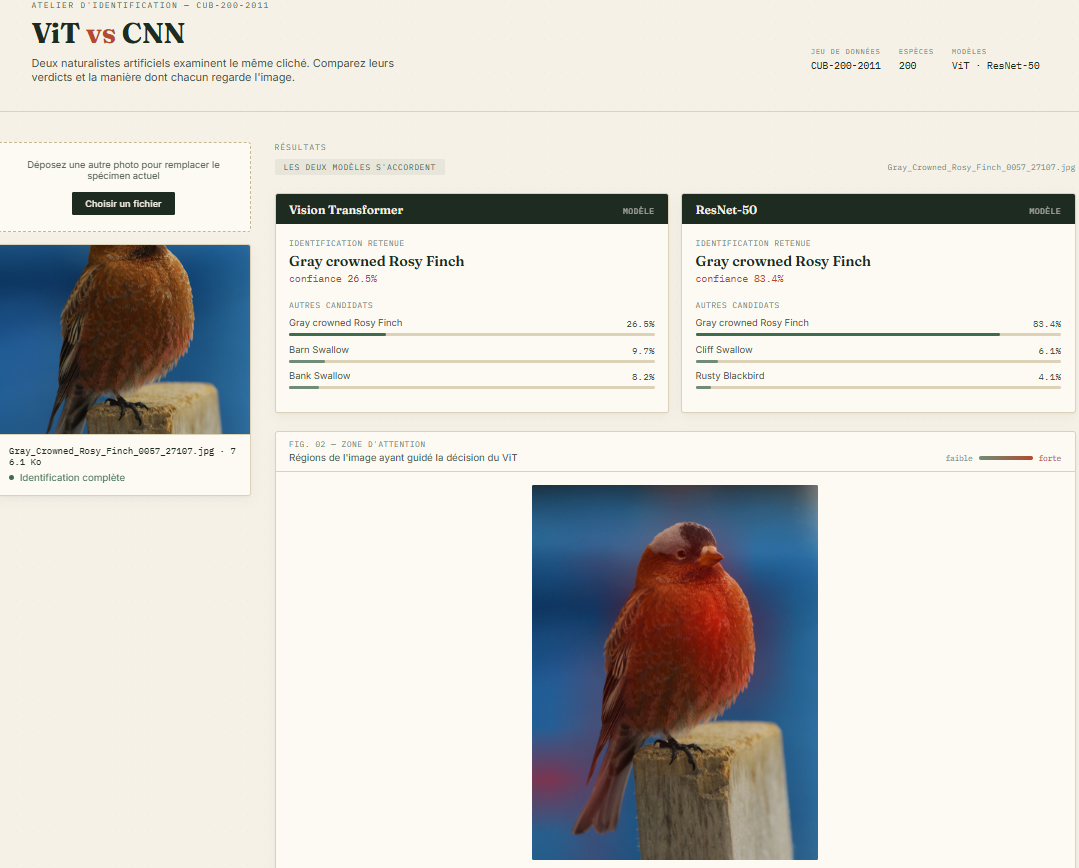
\includegraphics[width=\linewidth]{figures/app_nominal.png}
  \caption{Cas nominal : identification correcte et accord entre les deux modèles sur une image du jeu de test CUB-200-2011.}
  \label{fig:app_nominal}
\end{figure}

\begin{figure}[t]
  \centering
  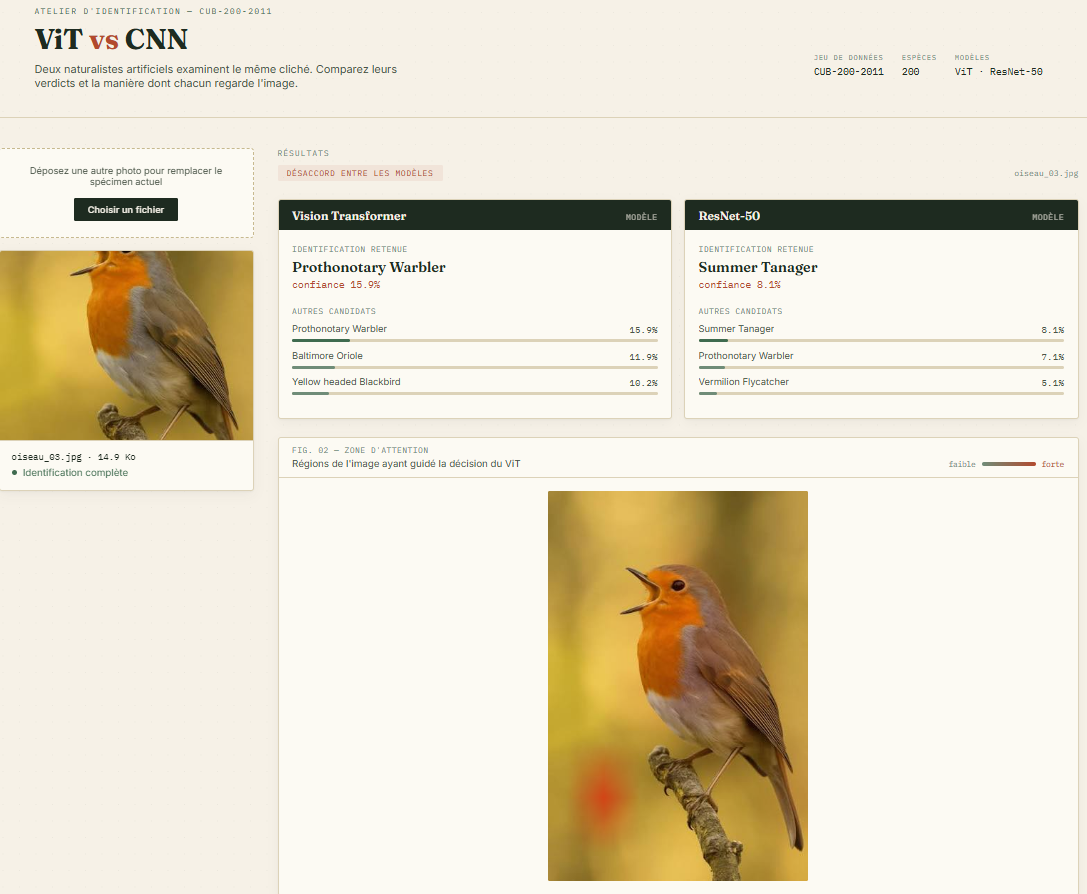
\includegraphics[width=\linewidth]{figures/app_ood.png}
  \caption{Cas hors distribution : une espèce absente du jeu d'entraînement (rouge-gorge européen) produit de faibles confiances et un désaccord entre les modèles.}
  \label{fig:app_ood}
\end{figure}
\section{Discussion et limites}
\label{sec:discussion}

\subsection{Synthèse des résultats}

Les résultats de ce projet confirment, sur une tâche de classification
fine-grained à petite échelle, le comportement data-hungry du ViT
documenté dans la littérature~\cite{dosovitskiy2020vit,touvron2021deit} :
sans pré-entraînement à grande échelle, le ViT n'apprend pas de
représentation exploitable dans les conditions expérimentales de ce
projet, quelle que soit la quantité de données d'entraînement fournie.
À l'inverse, ResNet-50 exploite efficacement son biais inductif
convolutif pour apprendre une représentation utile même avec 10\,\% du
jeu d'entraînement, et atteint 71{,}9\,\% de top-1 avec le jeu complet.
Le ViT pré-entraîné, quant à lui, confirme l'intérêt du pré-entraînement
à grande échelle : sa variante patch32 atteint 53{,}9\,\% de top-1,
là où le ViT from scratch reste bloqué au niveau du hasard.

L'application de démonstration développée pour ce projet illustre ce
contraste de manière concrète : sur une image test correctement
identifiée, ViT et ResNet-50 s'accordent avec des niveaux de confiance
cohérents ; sur une image hors distribution (espèce absente de
CUB-200-2011), les deux modèles produisent des confiances faibles et
sont en désaccord, un comportement souhaitable plutôt qu'une erreur
silencieuse (Section~\ref{sec:deployment}).

\subsection{Limites}

\textbf{Nombre d'epochs restreint.} Les modèles ont été entraînés sur
seulement 3 epochs (Section~\ref{sec:methodology}), une contrainte de
temps de calcul disponible sur la durée du projet. Cette limite affecte
en premier lieu le ViT from scratch, dont l'absence totale
d'apprentissage (accuracy proche du hasard indépendamment de la
quantité de données) est probablement davantage due à un
sous-entraînement qu'à une limite intrinsèque de l'architecture. Un
entraînement plus long, combiné à un scheduler de taux d'apprentissage
et à un arrêt anticipé (tous deux implémentés dans l'outil
d'entraînement du projet mais non encore appliqués aux résultats
rapportés), constituerait la première piste d'amélioration.

\textbf{Écart inexpliqué entre les variantes patch16 et patch32 du ViT
pré-entraîné.} La variante patch16 (9{,}9\,\% de top-1) performe
nettement moins bien que la variante patch32 (53{,}9\,\%), un résultat
contre-intuitif qui n'a pas pu être expliqué dans le temps imparti et
mériterait une investigation plus poussée (vérification du taux
d'apprentissage, du nombre d'itérations, ou d'un éventuel problème de
convergence spécifique à cette configuration).

\textbf{Échelle réduite du ViT from scratch.} L'implémentation
personnalisée du ViT (6 blocs, dimension d'embedding 384) reste
nettement plus petite que le ViT-Base original~\cite{dosovitskiy2020vit},
ce qui limite la portée des comparaisons avec les résultats publiés
dans la littérature.

\textbf{Absence de variance statistique.} Chaque configuration n'a été
entraînée qu'une seule fois (un seul seed), sans répétition pour
estimer la variance des résultats d'un run à l'autre.

\textbf{Taille du jeu de données.} Avec 5\,094 images d'entraînement,
CUB-200-2011 reste un jeu de données modeste au regard des standards
de pré-entraînement des Vision Transformers, ce qui limite la capacité
du ViT from scratch à démontrer son potentiel dans ce cadre expérimental.
\section{Répartition du travail}
\label{sec:contributions}

% Rôle C — à rédiger en toute fin de projet (Jour 13-14), une fois les
% contributions réelles de chacun connues.
%
% Format attendu : nom + rôle + contributions précises (pas juste
% "A a fait la partie données" mais le détail concret : quels scripts,
% quelles sections du rapport, quelles décisions techniques).

\begin{itemize}
  \item \textbf{Prénom Nom A} (Data / Experiment Engineer) : TODO — détailler.
  \item \textbf{Prénom Nom B} (Model / Research Engineer) : TODO — détailler.
  \item \textbf{Prénom Nom C} (Reporting / Backend Developer) : TODO — détailler.
\end{itemize}


\bibliographystyle{plain}
\bibliography{references}

\end{document}
